\usetikzlibrary{calc}
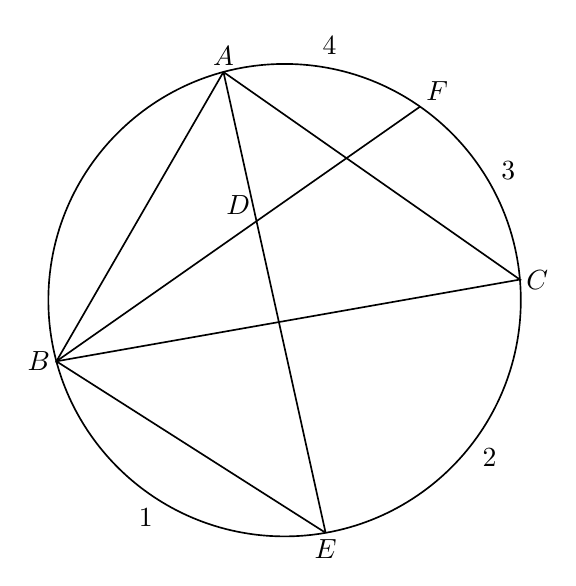
\begin{tikzpicture}[x=1cm,y=1cm,line width=.6pt,font=\normalsize]
\coordinate (O) at (0.0000,0.0000);
\coordinate (A) at (-0.7765,2.8978);
\coordinate (B) at (-2.8978,-0.7765);
\coordinate (C) at (2.9886,0.2615);
\coordinate (D) at (-0.3564,1.0030);
\coordinate (E) at (0.5209,-2.9544);
\coordinate (F) at (1.7207,2.4575);
\draw (O) circle[radius=3.0000];
\draw (A)--(B)--(C)--cycle;
\draw (A)--(E);
\draw (B)--(F);
\draw (B)--(E);
\node[above=2pt,inner sep=0pt] at (A) {$A$};
\node[left=2pt,inner sep=0pt] at (B) {$B$};
\node[right=2pt,inner sep=0pt] at (C) {$C$};
\node[above left=2pt,inner sep=0pt] at (D) {$D$};
\node[below=2pt,inner sep=0pt] at (E) {$E$};
\node[above right=2pt,inner sep=0pt] at (F) {$F$};
\node at (-1.76234272,-2.76632394) {$1$};
\node at (2.60219896,-1.99673749) {$2$};
\node at (2.84056332,1.64000000) {$3$};
\node at (0.56956602,3.23016943) {$4$};
\end{tikzpicture}
